\begin{slide}
  \begin{block}{Problem}
    Given a set of blue, red and green points in the plane, draw two
    polygons so that each color has its own region.
    
    \centering
\includegraphics[width=6cm]{sample}
  \end{block}
\end{slide}
\begin{slide}
  \begin{block}{Solution 1}
    \begin{itemize}
      \item Sort all points lexicographically, then go column by column.
      \item Draw the polygons in parallel, shifting left or right depending on color.
    \end{itemize}
    \centering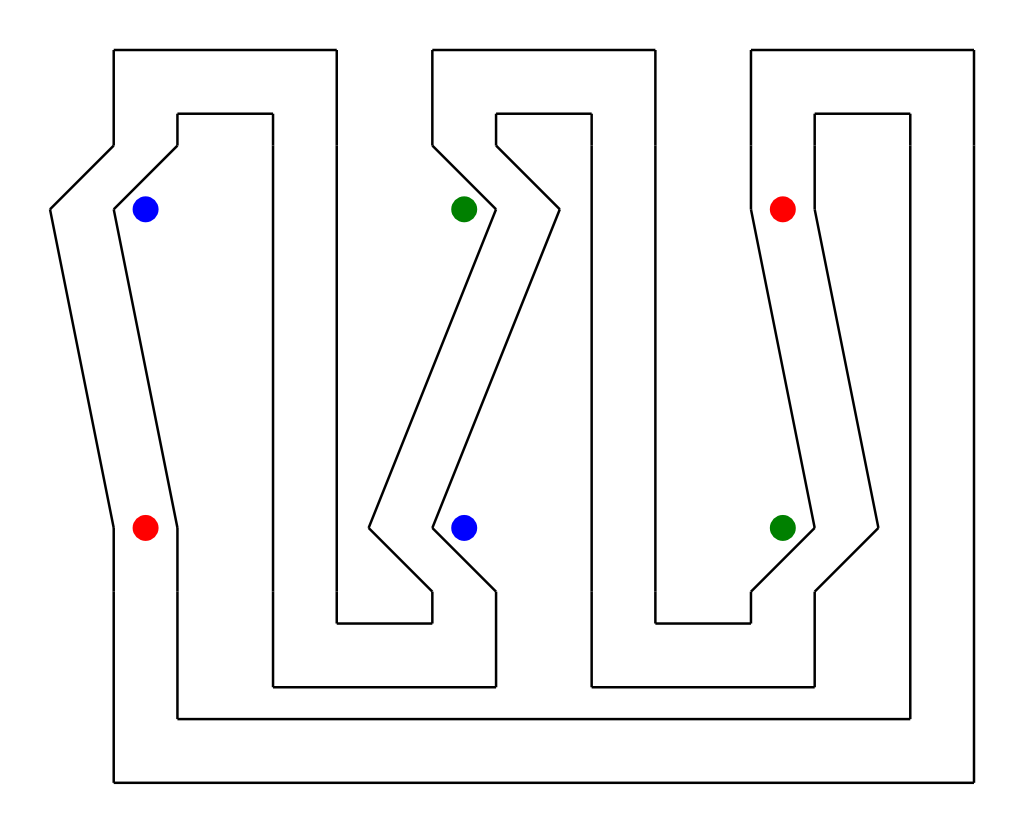
\includegraphics[width=6cm]{nested}
  \end{block}
\end{slide}
\begin{slide}
  \begin{block}{Solution 2}
    \begin{itemize}
      \item Sort all points lexicographically, then go column by column.
      \item Draw two comb-shaped polygons from top and bottom, adding
        protrusions to ``capture'' the appropriate color.
    \end{itemize}
    \centering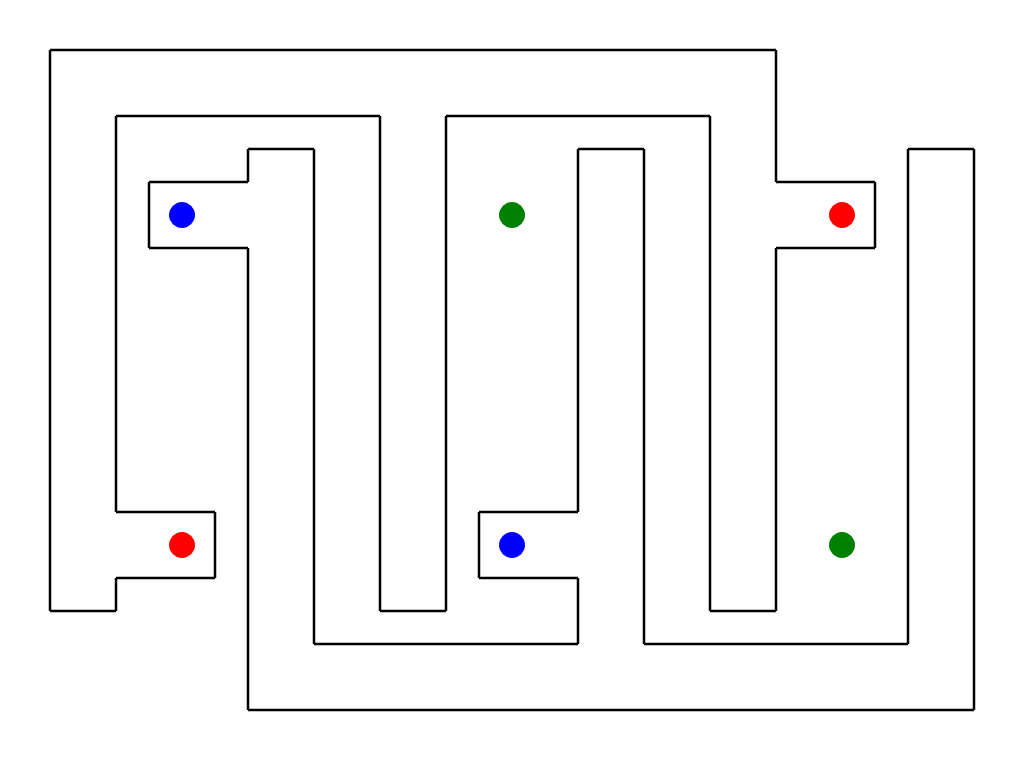
\includegraphics[width=6cm]{combs}
  \end{block}
\end{slide}
\begin{slide}
  \begin{block}{Solution 3}
    \begin{itemize}
      \item Pick a direction at random and do a zigzag in that direction.
    \end{itemize}
    \centering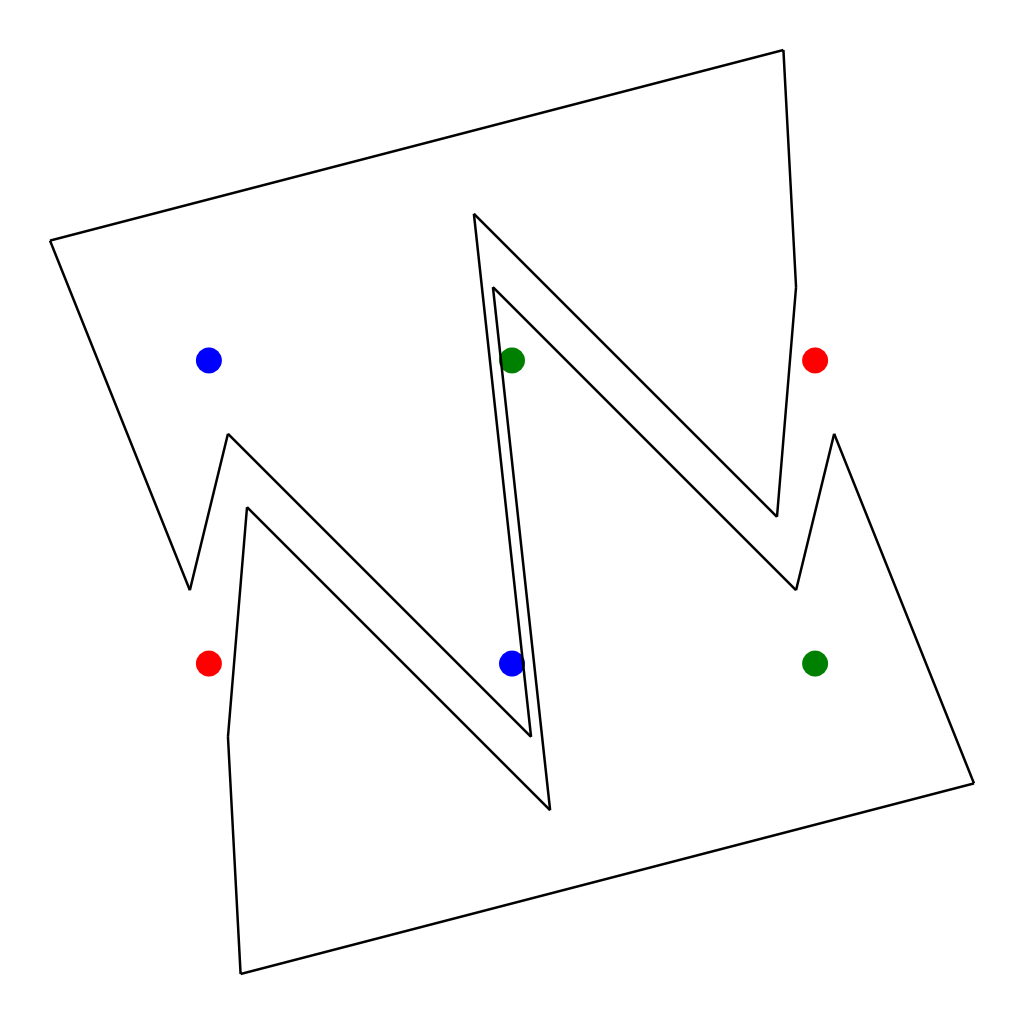
\includegraphics[width=6cm]{rand}
  \end{block}
\end{slide}
